Near threshold, we find
\begin{align}
c_{\vec k,\Pq}^{(1),\tThr} &= c_{\vec k,\Pg}^{(0),\text{thr}} \frac{\beta^2\rho_q}{\pi^2(\rho_q-1)} \frac{K_{\Pq\Pgg}}{6K_{\Pg\Pgg}} \left[a_{\vec k,\Pq}^{(1,1)}\ln(\beta) + a_{\vec k,\Pq}^{(1,0)}\right],
\end{align}
with
\begin{align}
a^{(1,1)}_{\tVV,F_2,\Pq} &= 1\\
a^{(1,1)}_{\tVV,F_L,\Pq} &= a^{(1,1)}_{\tVV,F_2,\Pq} - \frac 2 {3}\\
a^{(1,1)}_{\tVV,2xg_1,\Pq} &= a^{(1,1)}_{\tAA,F_2,\Pq} = a^{(1,1)}_{\tAA,F_L,\Pq} = a^{(1,1)}_{\tAA,2xg_1,\Pq}= a^{(1,1)}_{\tVV,F_2,\Pq}\\
a^{(1,0)}_{\tVV,F_2,\Pq} &= -\frac{13}{12} + \frac 3 2 \ln(2)\\
a^{(1,0)}_{\tVV,F_L,\Pq} &= -\frac{77}{100} + \frac 9 {10} \ln(2) \\
a^{(1,0)}_{\tVV,2xg_1,\Pq} &= a^{(1,0)}_{\tVV,F_2,\Pq} - \frac{1}{4}\\
a^{(1,0)}_{\tAA,F_2,\Pq} &= a^{(1,0)}_{\tAA,F_L,\Pq} = a^{(1,0)}_{\tAA,2xg_1,\Pq}= a^{(1,0)}_{\tVV,F_2,\Pq}
\end{align}

\begin{figure}[ht!]
\centering
\begin{subfigure}[t]{.3\textwidth}
	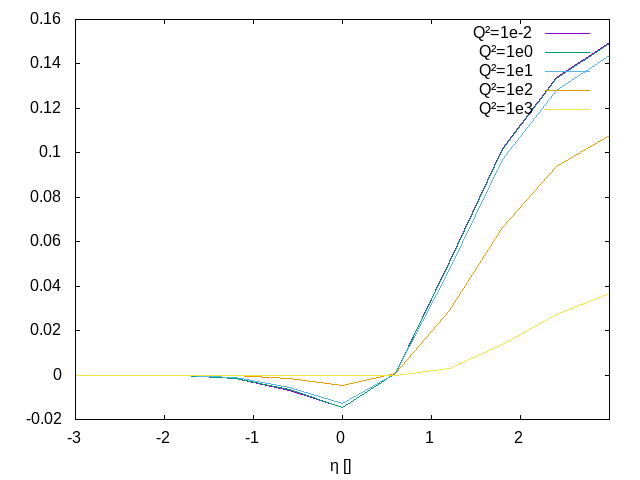
\includegraphics[width=\textwidth]{../../img2/partonic/cq1_VV_F2}
\end{subfigure}%
\begin{subfigure}[t]{.3\textwidth}
	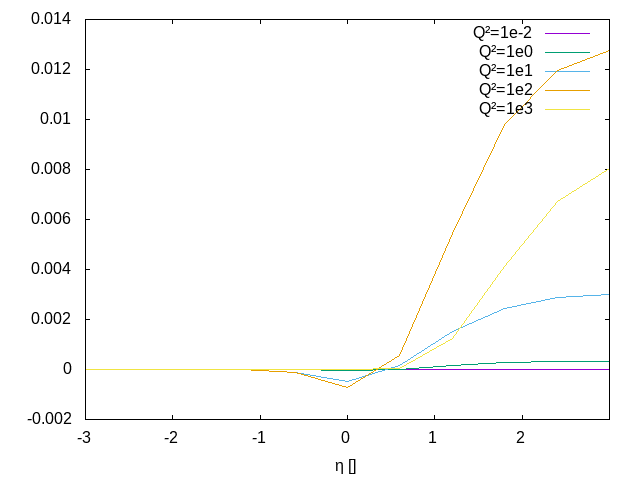
\includegraphics[width=\textwidth]{../../img2/partonic/cq1_VV_FL}
\end{subfigure}%
\begin{subfigure}[t]{.3\textwidth}
	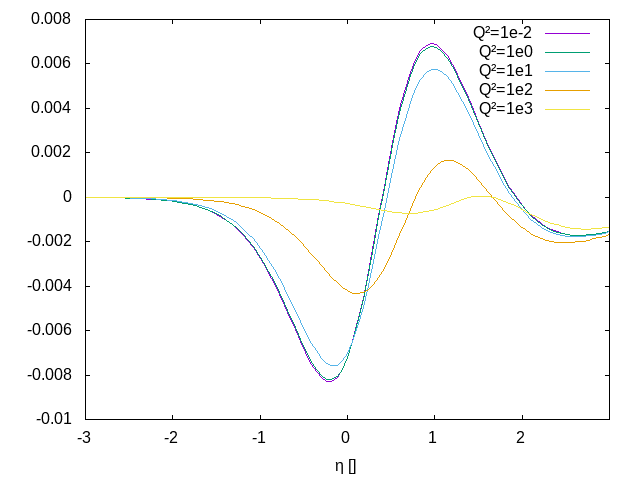
\includegraphics[width=\textwidth]{../../img2/partonic/cq1_VV_x2g1}
\end{subfigure}\\%
\begin{subfigure}[t]{.3\textwidth}
	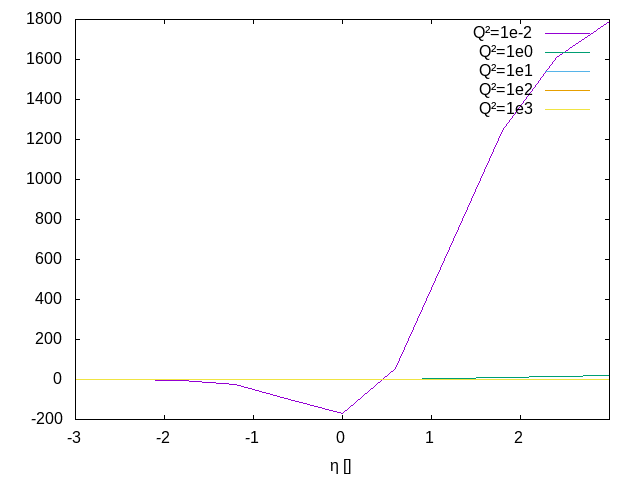
\includegraphics[width=\textwidth]{../../img2/partonic/cq1_AA_F2}
\end{subfigure}%
\begin{subfigure}[t]{.3\textwidth}
	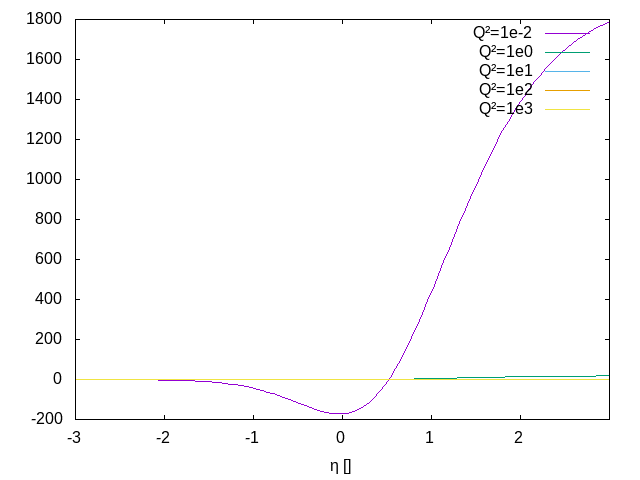
\includegraphics[width=\textwidth]{../../img2/partonic/cq1_AA_FL}
\end{subfigure}%
\begin{subfigure}[t]{.3\textwidth}
	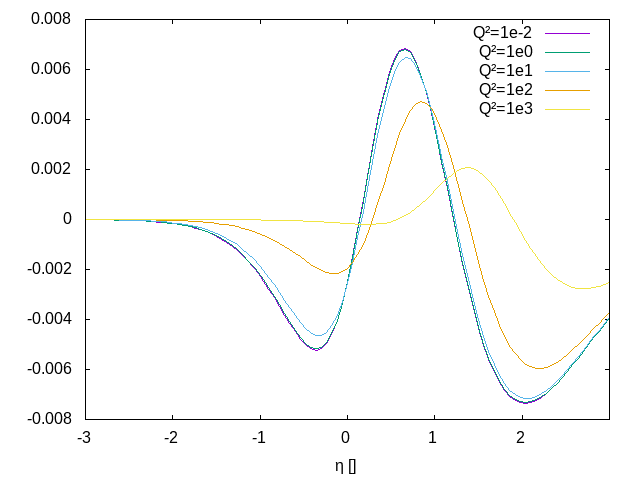
\includegraphics[width=\textwidth]{../../img2/partonic/cq1_AA_x2g1}
\end{subfigure}%
\caption{next-to-leading order scaling functions $c_{k,\Pq}^{(1)}(\eta,\xi)$ plotted as function of $\eta=s/(4m^2)-1$ for different values of $Q^2$ in units of $\si{\GeV^2}$ at $m=\SI{4.75}{\GeV}$ (i.e. different values of $\xi=Q^2/m^2$) }\label{fig:cq1}
\end{figure}
